\chapter{Prototypische Implementierung}
\label{chap:impl}

Our prototypic implementation of the introduced models shows, the applicability of this optimization approach to a channel based publish/subscribe system. We choose C++ as language of choice and we use Chimera \cite{Allen2006Chimera}, a structured p2p-overlay system written in C. In order to minimize the overhead introduced by the flexibility of such a framework e.g. on message size or stack depth caused by function calls, we use \ac{tmp} and \emph{policy based}-design \cite{Alexandrescu2001Modern} to create the optimized channels at compile-time. The different optimization strategies for each dimension are implemented as policies encapsulating their behaviour. Each channel is therefore a template class with all dimensions as template parameters, which are instantiated with strategies for each parameter.  

With \ac{tmp} it is possible to derive create custom-tailored message headers, depending on the chosen strategies. This ensures small message sizes with a high payload ratio. Each channel itself is therefore in charge to orchestrate strategies for the different policies with regard to our processing model, derived by the semantic description for all optimization dimensions. All described design decisions ensure that the system has a small footprint at runtime and that it can be used without further knowledge of the system internals, the channels or the used strategies.

\section{Moderne Entwicklung mit C++}
\label{chap:impl_tmp}
\acf{tmp}\index{Template Meta-Programming} und policy-based Design\index{policy-based Design} \cite{Alexandrescu2001Modern} sind Paradigmen der Softwareentwicklung in C++ und bedienen sich der dort verfügbaren \emph{Templates}. Policy-based Design baut in der hier erklärten Variante auf dem turingvollständigem \ac{tmp} auf.

\subsection{Templates}
Templates dienen der Generalisierung von Code und werden zur Übersetzungszeit durch den Compiler ausgewertet. Templates sind ein integraler Bestandteil der \ac{stl}\footnote{Siehe auch \url{http://www.cplusplus.com/reference/stl/}} und dienen dort vor Allem zum Erstellen von abstrakten Containerklassen wie zum Beispiel \texttt{std::vector}, \texttt{std::map} oder \texttt{std::set}. Basierend auf dem Konzept des Zugriffs über \texttt{Iteratoren}, sind viele aus der Funktionalen Programmierung bekannte Funktionen implementiert, die ebenfalls durch Templates generisch gehalten sind.

Einzelne Funktionen oder komplette Klassen könnten als Template realisiert werden. Zusätzlich der generischen Implementierung können auch spezielle Implementierungen, sog. Spezialisierungen, angegeben werden können. Funktionstemplates lassen sich nur total, Klassentemplates auch partiell spezialisieren. Eine partielle Spezialisierung kann bei mehreren Templateparametern erfolgen. Ungenutzte Templates werden vom Compiler nicht instantiiert, dies bedeutet dass kein ungenutzter Code im fertigem Kompilat vorhanden ist. Dies wiederum verringert die Größe von ausführbaren Dateien oder dynamischen Bibliotheken. Jedoch muss erwähnt werden, dass jede Instanz eines Templates eigenen Code generiert. Dieser lässt sich - dank des Wissens zur Übersetzungszeit - besser optimieren als zur Laufzeit.

In diesem und den folgenden Beispielen soll ein Einblick in die neue Methodik gezeigt werden, daher wird nicht auf eine optimierte Parameterübergabe oder Ähnliches geachtet. \Fref{lst:tmp_easy_spez} zeigt ein einfaches Template. Der Funktion \texttt{min} wird als Templateparameter der Typ der Parameter übergeben. Es wird erwartet, dass die übergebenen Typen den Operator $<$ überladen haben. Für den Typ \texttt{Pair} ist das Template total spezialisiert und eine separate Implementierung wurde angegeben. Zeilen 18 und 19 zeigen die einzelnen Funktionsaufrufe.

\lstinputlisting[caption={einfaches Funktionstemplate}, label=lst:tmp_easy_spez, float=t]{listings/tmp_easy_spez.cpp}

Ebenso können Templates geschachtelt übergeben werden, wie es \Fref{lst:tmp_tmp} zeigt. Hier wird dem \texttt{WidgetFactory} ein Template übergeben mit dessen Hilfe er Objekte des Typs \texttt{Widget} erstellen kann. Beim Aufruf in Zeile 19 muss der Entwickler dennoch Typ angeben obwohl eine \texttt{WidgetFactory} nur Objekte des Typs \texttt{Widget} erzeugt, wie es der Name impliziert.

\lstinputlisting[caption={einfaches Klassentemplate}, label=lst:tmp_tmp, float=t]{listings/tmp_tmp.cpp}

\Fref{lst:tmp_tmp_2} zeigt die Lösung mit \enquote{Template Template} Parametern. Hier wird der \texttt{WidgetFactory} ein Template übergeben. Dieses Template ist noch nicht spezifiziert und benötigt weiterhin den Typ des zu erstellenden Objektes. Der Unterschied zum vorherigem Listing ist in Zeile 5 und am Aufruf in Zeile 10 zu sehen. \texttt{WidgetFactory} übergibt den Typ an das Template. Der Entwickler ist nicht mehr für die Auswahl des korrekten Typs zuständig.

\lstinputlisting[caption={verbessertes Klassentemplate mit Template Template}, label=lst:tmp_tmp_2, float=!t]{listings/tmp_tmp_2.cpp}

Mit Templates lassen sich auch Entscheidungen anhand der übergebenen Templateparamter treffen. In \Fref{lst:tmp_cond} wird anhand des Parameters \texttt{isSingleton} entschieden, ob das neue Objekt mit \texttt{new} oder per Aufruf der Methode \texttt{T::getInstance()} erzeugt werden kann.

\lstinputlisting[caption={Entscheidung via Templates}, label=lst:tmp_cond, float=t]{listings/tmp_cond.cpp}

Der Compiler prüft dabei alle Templates syntaktisch. Obwohl \texttt{isSingleton} mit \texttt{false} instantiert wird, kann der Code nicht kompiliert werden, denn die Methode \texttt{getInstance} wird von \emph{Foo} nicht angeboten. Um dieses Problem zu umgehen, beschreibt Alexandrescu in \cite{Alexandrescu2001Modern} das Hilfskonstrukt \texttt{Int2Type} das im nächsten Kapitel eingeführt wird.

\subsection{Template Meta-Programming}
Template Meta-Programming arbeitet mit der vorgestellten Spezialisierung von Templates und wird ebenfalls vom Compiler zum Übersetzungszeitpunkt ausgewählt und basiert rein auf Typinformation.

\ac{tmp} kann dazu genutzt werden, um die Problematik im vorangegangenen Kapitel zu lösen. \Fref{lst:tmp_cond_2} zeigt die Definition von \texttt{Int2Type}. \texttt{Int2Type} speichert den übergebenen Integerwert und erzeugt daraus pro Wert einen eigenen Typ. Mit überladenen Funktionen kann nun eine Auswahl zur Übersetzungszeit erfolgen. Die statische Methode \texttt{create} (Zeile 8) ruft nun abhängig vom Templateparameter \texttt{isSingleton} die überladene Methode \texttt{create\_impl} auf. Im ersten Fall (Zeile 14) nimmt diese ein \texttt{Int2Type$<$true$>$}, im zweiten Falle (Zeile 19) nur \texttt{Int2Type$<$false$>$}. Da der Compiler nur instantiierte Templates prüfen muss, gibt es nun keine Übersetzungsfehler mehr. Der Entwickler muss seinen Aufruf nicht anpassen.

\lstinputlisting[caption={Entscheidung via Templates zur Übersetzungzeit}, label=lst:tmp_cond_2, float=t]{listings/tmp_cond_2.cpp}

Durch diese Technik können Entscheidungen zur Übersetzungszeit getroffen werden. So können zum Beispiel auch komplexe Berechnungen zur Übersetzungszeit ein- beziehungsweise ausgeschaltet werden. Der zusätzliche Code (zum Beispiel Methodenaufruf) kann durch den Compiler leicht optimiert werden.

\subsection{Policy-based Design}
Policy-based Design kombiniert Vererbung und Templates und ermöglicht es generischen Code zu entwickeln. Hierbei lassen sich sehr gut orthogonale Aspekte ausnutzen, wie Alexandrescu am Beispiel eines SmartPointers erläutert.

In \Fref{lst:tmp_pbd} ist ein einfaches Beispiel mit einer Ausgabeklasse (\emph{Ausgabe}) beschrieben, die mittels einem \emph{Decorator} und einem \emph{Printer} parametrisiert wird. Ausgabe leitet von diesen beiden Typen ab und nutzt deren Funktionalität. Dadurch erzeugt der Compiler implizit Anforderungen die diese Parameter zu erfüllen haben. Jeder Decorator muss eine Methode \texttt{decorate} anbieten, welche einen \emph{const string\&} als Parameter nimmt. Jeder Printer muss eine Methode \texttt{print} anbieten, welche den Rückgabetyp von Decorator::decorate als Parameter nimmt. Diese Kontrakte werden vom Compiler zur Übersetzungszeit in Zeile 24 geprüft. Weitere Varianten für Decorator und Printer sind trivial.

Ausgabe wird in diesem Zusammenhang als \enquote{Host-Klasse}, Dec\_A und Printer als \enquote{Policy-Klasse} bezeichnet. Da die Host-Klasse von ihren Policy-Klassen ableitet, kann die Host-Klasse in eine Policy-Klasse gecastet werden. So können nützliche Informationen abgefragt oder speziell angepasste Methoden der Policy-Klasse aufgerufen werden. Der Nutzer einer solchen mit Policies angereicherten Klasse bekommt dadurch sehr viele Freiheiten. Mögliche Sonderfälle spricht Aleandrescu an und bietet angepasste Lösungen.

\lstinputlisting[caption={Beispiel für policy-based Design}, label=lst:tmp_pbd, float=t]{listings/tmp_pbd.cpp}

Diese Möglichkeit der Parametrisierung vom Klassen gibt es prinzipell auch zur Laufzeit. Hier wird jede Policy durch einen Pointer auf eine abstrakte Basisklasse abgebildet. Jedoch hat dies einige Nachteile zur Laufzeit. Zum einen sind die Interfaces der Policy-Klassen festgeschrieben und die Host-Klasse leitet nicht von diesen ab. Zusätzlich sind virtuelle Funktionsaufrufe \enquote{teuer}, da diese in der sogenannten \enquote{VTable} zur Laufzeit abgeprüft werden müssen. Diese Überprüfung kann durch den Compiler nicht entfernt oder optimiert werden. 


In dieser Arbeit kommt \ac{tmp} im Zusammenspiel mit policy-based Design bei der Entwicklung des einzelnen Kanals zur Anwendung. Durch die Optimierungen zur Übersetzungszeit wird schlanker Code ohne unnötigen Ballast zur Laufzeit erzeugt.


\section{Implementierungsdetails}

\begin{figure}[htbp]
\centering
\resizebox{\textwidth}{!}{%
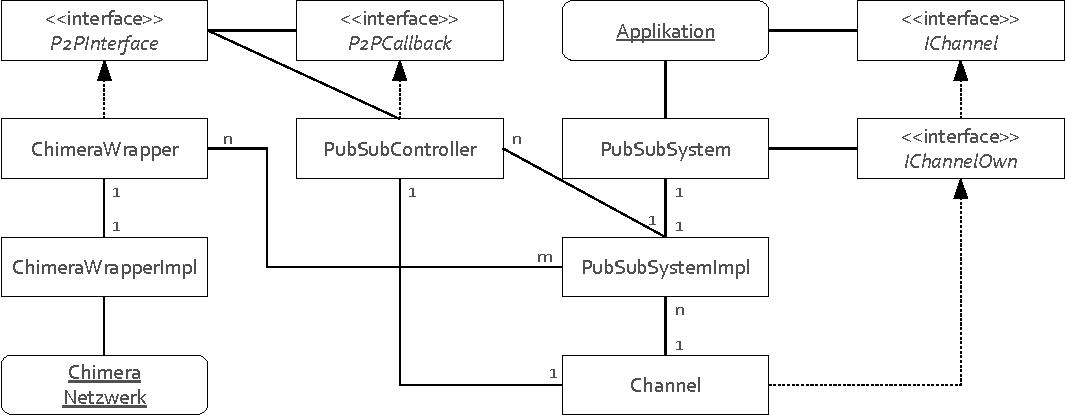
\includegraphics{grafics/uml.pdf}}
\caption{vereinfachtes Klassendiagramm des Frameworks}
\label{fig:uml}
\end{figure}

\emph{P2PInterface} ist eine abstrakte Basisklasse und repräsentiert die in \cite{Dabek2003Towards} beschrieben KBR-API. Aktuell wird diese vom \emph{ChimeraWrapper} implementiert, der über den \emph{ChimeraWrapperImpl} mit dem Netzwerk Chimera spricht. Hier wurde das ``PIMPL''-Pattern angewandt, mit dem die eigentliche Implementierung versteckt werden kann \cite{Alexandrescu2001Modern}. Die \emph{Applikation} spricht mit dem \emph{PubSubSytem}, dessen Implementierung auch in einer eigenen Klasse ausgelagert ist. Die Applikation und das PubSubSystem kennen den \emph{Channel} nur über die abstrakte Basisklasse \emph{IChannel} beziehungsweise \emph{IChannelOwn}. Durch diese beiden Basisklassen wird die Komplexität der durch Policies optimierten Klasse Channel verdeckt. Die Klasse \emph{PubSubController} implementiert das Interface \emph{P2PCallback} und kann sich somit für die Callbacks des Netzwerkes registrieren. Weiterhin bietet diese Klasse die von Channel benötigte Funktionalität. PubSubSystemImpl kennt die Netzwerkwrapperklassen (in \Fref{fig:uml} ChimeraWrapper) und verbindet diese über den PubSubController mit dem Channel. Mit verschiedene Instanzen des PubSubControllers können somit auch verschiedene Netzwerke angesprochen werden und entsprechend der Optimierung für verschiedene Channel eingesetzt werden.

\subsection{Netzwerkabstraktion}
\begin{itemize*}
\item Abstrakte Basisklasse für Netzwerk
\item Abstrakte Basisklasse für Netzwerkupcalls
\item Wrapperklassen für jedes Netzwerk
\end{itemize*}


\subsection{PubSubabstraktion}
\begin{itemize*}
\item PubSubController spricht mit Netzwerk
\item PubSubSystem spricht mit Applikation und leitet Anfragen an Channel weiter
\item Channel nutzt Controller zum Netzwerkzugriff
\item $\rightarrow$ Möglichkeit verschiedene Netzwerke zu nutzen!
\end{itemize*}

\subsection{Channel}
\begin{itemize*}
\item Channel mit TMP und policy-based Design
\item viele verschiedene Strategien
\end{itemize*}

\lstinputlisting[caption={\ac{m2etis} aus Benutzersicht}, label=lst:pubsub_usage]{listings/pubsub_usage.cpp}
